\documentclass[12pt]{standalone}

\usepackage{tikz}

\begin{document}
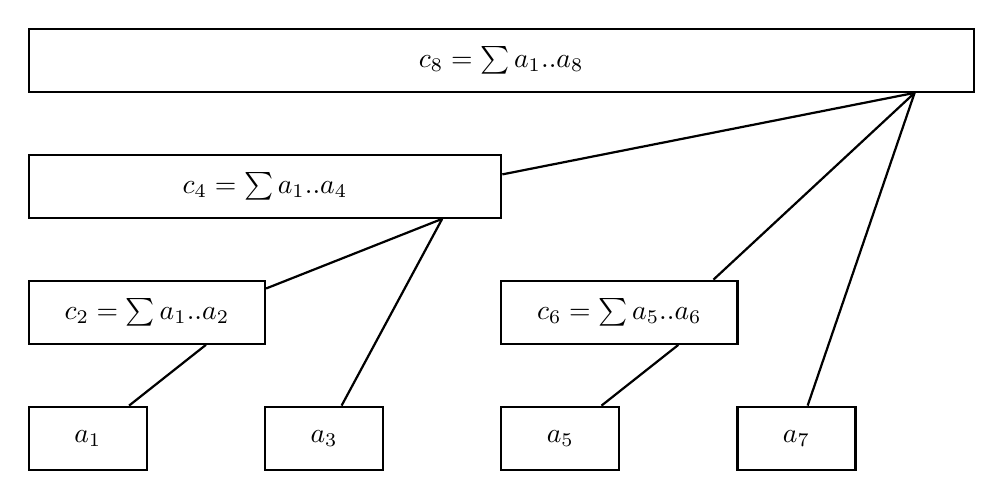
\begin{tikzpicture}[x=15mm,y=8mm,thick,
    every node/.style={minimum width=15mm,minimum height=8mm}]

\draw (0,1) rectangle node (c1) {$a_1$} (1,0);
\draw (2,1) rectangle node (c3) {$a_3$} (3,0);
\draw (4,1) rectangle node (c5) {$a_5$} (5,0);
\draw (6,1) rectangle node (c7) {$a_7$} (7,0);

\draw (0,3) rectangle node {$c_2 = \sum a_1 .. a_2$} (2,2);
\node (c2) at (1.5,2.5) {};
\draw (4,3) rectangle node {$c_6 = \sum a_5 .. a_6$} (6,2);
\node (c6) at (5.5,2.5) {};

\draw (0,5) rectangle node {$c_4 = \sum a_1 .. a_4$} (4,4);
\node (c4) at (3.5,4.5) {};

\draw (0,7) rectangle node {$c_8 = \sum a_1 .. a_8$} (8,6);
\node (c8) at (7.5,6.5) {};

\path (c2.south) edge (c1)
    (c4.south) edge (c3)
    (c6.south) edge (c5)
    (c8.south) edge (c7)
    (c4.south) edge (c2)
    (c8.south) edge (c6)
    (c8.south) edge (c4);

\end{tikzpicture}
\end{document}
